\documentclass[aspectratio=169,t]{beamer}
\usepackage{slides}

% Define `accent`/`accent2` colors for theme customization:
\definecolor{accent}{HTML}{006896}
\definecolor{accent2}{HTML}{695693}

\title{What is the Effect of X on Y?}
\date{\today}
\author{Kyle Butts}

% \addbibresource{references.bib}
\begin{document}

% ------------------------------------------------------------------------------
\begin{frame}
\maketitle

% \vspace{2.5mm}
% {\footnotesize $^*$ A bit of extra info here. Add an asterich to title or author}
\end{frame}
% ------------------------------------------------------------------------------

\section{Motivation}

\begin{frame}[plain,c]
  % Created by tikzDevice version 0.12.6 on 2024-07-30 16:24:38
% !TEX encoding = UTF-8 Unicode
\begin{tikzpicture}[x=1pt,y=1pt]
\definecolor{fillColor}{RGB}{255,255,255}
\path[use as bounding box,fill=fillColor] (0,0) rectangle (433.62,216.81);
\begin{scope}
\path[clip] (  0.00,  0.00) rectangle (433.62,216.81);
\definecolor{drawColor}{RGB}{255,255,255}

\path[draw=drawColor,line width= 0.5pt,line join=round,line cap=round,fill=fillColor] (  0.00,  0.00) rectangle (433.62,216.81);
\end{scope}
\begin{scope}
\path[clip] ( 54.74, 28.35) rectangle (417.62,200.81);
\definecolor{drawColor}{RGB}{255,255,255}
\definecolor{fillColor}{RGB}{255,255,255}

\path[draw=drawColor,line width= 0.5pt,line join=round,line cap=round,fill=fillColor] ( 54.74, 28.35) rectangle (417.62,200.81);
\definecolor{drawColor}{RGB}{209,213,219}

\path[draw=drawColor,line width= 0.4pt,line join=round] ( 54.74, 54.59) --
	(417.62, 54.59);

\path[draw=drawColor,line width= 0.4pt,line join=round] ( 54.74, 92.09) --
	(417.62, 92.09);

\path[draw=drawColor,line width= 0.4pt,line join=round] ( 54.74,129.58) --
	(417.62,129.58);

\path[draw=drawColor,line width= 0.4pt,line join=round] ( 54.74,167.07) --
	(417.62,167.07);

\path[draw=drawColor,line width= 0.4pt,line join=round] ( 54.74, 35.85) --
	(417.62, 35.85);

\path[draw=drawColor,line width= 0.4pt,line join=round] ( 54.74, 73.34) --
	(417.62, 73.34);

\path[draw=drawColor,line width= 0.4pt,line join=round] ( 54.74,110.83) --
	(417.62,110.83);

\path[draw=drawColor,line width= 0.4pt,line join=round] ( 54.74,148.32) --
	(417.62,148.32);

\path[draw=drawColor,line width= 0.4pt,line join=round] ( 54.74,185.81) --
	(417.62,185.81);

\path[draw=drawColor,line width= 0.4pt,line join=round] ( 73.56, 28.35) --
	( 73.56,200.81);

\path[draw=drawColor,line width= 0.4pt,line join=round] (120.02, 28.35) --
	(120.02,200.81);

\path[draw=drawColor,line width= 0.4pt,line join=round] (166.49, 28.35) --
	(166.49,200.81);

\path[draw=drawColor,line width= 0.4pt,line join=round] (212.95, 28.35) --
	(212.95,200.81);

\path[draw=drawColor,line width= 0.4pt,line join=round] (259.41, 28.35) --
	(259.41,200.81);

\path[draw=drawColor,line width= 0.4pt,line join=round] (305.88, 28.35) --
	(305.88,200.81);

\path[draw=drawColor,line width= 0.4pt,line join=round] (352.34, 28.35) --
	(352.34,200.81);

\path[draw=drawColor,line width= 0.4pt,line join=round] (398.80, 28.35) --
	(398.80,200.81);
\definecolor{drawColor}{gray}{0.70}

\path[draw=drawColor,line width= 2.3pt,line join=round] ( 73.56,172.61) --
	(120.02,128.46) --
	(166.49,132.56) --
	(212.95,123.89) --
	(259.41,103.38) --
	(305.88,116.27) --
	(352.34,119.73) --
	(398.80,115.13);
\definecolor{drawColor}{gray}{0.40}

\path[draw=drawColor,line width= 2.3pt,line join=round] ( 73.56,156.29) --
	(120.02,119.42) --
	(166.49,120.91) --
	(212.95,111.28) --
	(259.41, 88.31) --
	(305.88,101.57) --
	(352.34, 99.76) --
	(398.80, 93.64);
\definecolor{drawColor}{gray}{0.10}

\path[draw=drawColor,line width= 2.3pt,line join=round] ( 73.56, 80.61) --
	(120.02, 93.11) --
	(166.49, 83.59) --
	(212.95, 69.34) --
	(259.41, 63.94) --
	(305.88, 56.30) --
	(352.34, 49.97) --
	(398.80, 54.06);
\definecolor{drawColor}{gray}{0.70}

\path[draw=drawColor,line width= 1.7pt,line join=round] ( 71.24,190.54) --
	( 75.88,190.54);

\path[draw=drawColor,line width= 1.7pt,line join=round] ( 73.56,190.54) --
	( 73.56,155.28);

\path[draw=drawColor,line width= 1.7pt,line join=round] ( 71.24,155.28) --
	( 75.88,155.28);
\definecolor{drawColor}{gray}{0.40}

\path[draw=drawColor,line width= 1.7pt,line join=round] ( 71.24,172.81) --
	( 75.88,172.81);

\path[draw=drawColor,line width= 1.7pt,line join=round] ( 73.56,172.81) --
	( 73.56,140.29);

\path[draw=drawColor,line width= 1.7pt,line join=round] ( 71.24,140.29) --
	( 75.88,140.29);
\definecolor{drawColor}{gray}{0.10}

\path[draw=drawColor,line width= 1.7pt,line join=round] ( 71.24, 94.64) --
	( 75.88, 94.64);

\path[draw=drawColor,line width= 1.7pt,line join=round] ( 73.56, 94.64) --
	( 73.56, 67.04);

\path[draw=drawColor,line width= 1.7pt,line join=round] ( 71.24, 67.04) --
	( 75.88, 67.04);
\definecolor{drawColor}{gray}{0.70}

\path[draw=drawColor,line width= 1.7pt,line join=round] (117.70,140.59) --
	(122.34,140.59);

\path[draw=drawColor,line width= 1.7pt,line join=round] (120.02,140.59) --
	(120.02,116.64);

\path[draw=drawColor,line width= 1.7pt,line join=round] (117.70,116.64) --
	(122.34,116.64);
\definecolor{drawColor}{gray}{0.40}

\path[draw=drawColor,line width= 1.7pt,line join=round] (117.70,130.77) --
	(122.34,130.77);

\path[draw=drawColor,line width= 1.7pt,line join=round] (120.02,130.77) --
	(120.02,108.35);

\path[draw=drawColor,line width= 1.7pt,line join=round] (117.70,108.35) --
	(122.34,108.35);
\definecolor{drawColor}{gray}{0.10}

\path[draw=drawColor,line width= 1.7pt,line join=round] (117.70,105.32) --
	(122.34,105.32);

\path[draw=drawColor,line width= 1.7pt,line join=round] (120.02,105.32) --
	(120.02, 81.23);

\path[draw=drawColor,line width= 1.7pt,line join=round] (117.70, 81.23) --
	(122.34, 81.23);
\definecolor{drawColor}{gray}{0.70}

\path[draw=drawColor,line width= 1.7pt,line join=round] (164.16,145.17) --
	(168.81,145.17);

\path[draw=drawColor,line width= 1.7pt,line join=round] (166.49,145.17) --
	(166.49,120.28);

\path[draw=drawColor,line width= 1.7pt,line join=round] (164.16,120.28) --
	(168.81,120.28);
\definecolor{drawColor}{gray}{0.40}

\path[draw=drawColor,line width= 1.7pt,line join=round] (164.16,132.12) --
	(168.81,132.12);

\path[draw=drawColor,line width= 1.7pt,line join=round] (166.49,132.12) --
	(166.49,109.97);

\path[draw=drawColor,line width= 1.7pt,line join=round] (164.16,109.97) --
	(168.81,109.97);
\definecolor{drawColor}{gray}{0.10}

\path[draw=drawColor,line width= 1.7pt,line join=round] (164.16, 95.22) --
	(168.81, 95.22);

\path[draw=drawColor,line width= 1.7pt,line join=round] (166.49, 95.22) --
	(166.49, 72.28);

\path[draw=drawColor,line width= 1.7pt,line join=round] (164.16, 72.28) --
	(168.81, 72.28);
\definecolor{drawColor}{gray}{0.70}

\path[draw=drawColor,line width= 1.7pt,line join=round] (210.63,134.79) --
	(215.27,134.79);

\path[draw=drawColor,line width= 1.7pt,line join=round] (212.95,134.79) --
	(212.95,113.24);

\path[draw=drawColor,line width= 1.7pt,line join=round] (210.63,113.24) --
	(215.27,113.24);
\definecolor{drawColor}{gray}{0.40}

\path[draw=drawColor,line width= 1.7pt,line join=round] (210.63,121.87) --
	(215.27,121.87);

\path[draw=drawColor,line width= 1.7pt,line join=round] (212.95,121.87) --
	(212.95,100.92);

\path[draw=drawColor,line width= 1.7pt,line join=round] (210.63,100.92) --
	(215.27,100.92);
\definecolor{drawColor}{gray}{0.10}

\path[draw=drawColor,line width= 1.7pt,line join=round] (210.63, 81.37) --
	(215.27, 81.37);

\path[draw=drawColor,line width= 1.7pt,line join=round] (212.95, 81.37) --
	(212.95, 57.66);

\path[draw=drawColor,line width= 1.7pt,line join=round] (210.63, 57.66) --
	(215.27, 57.66);
\definecolor{drawColor}{gray}{0.70}

\path[draw=drawColor,line width= 1.7pt,line join=round] (257.09,113.77) --
	(261.74,113.77);

\path[draw=drawColor,line width= 1.7pt,line join=round] (259.41,113.77) --
	(259.41, 93.24);

\path[draw=drawColor,line width= 1.7pt,line join=round] (257.09, 93.24) --
	(261.74, 93.24);
\definecolor{drawColor}{gray}{0.40}

\path[draw=drawColor,line width= 1.7pt,line join=round] (257.09, 98.81) --
	(261.74, 98.81);

\path[draw=drawColor,line width= 1.7pt,line join=round] (259.41, 98.81) --
	(259.41, 78.05);

\path[draw=drawColor,line width= 1.7pt,line join=round] (257.09, 78.05) --
	(261.74, 78.05);
\definecolor{drawColor}{gray}{0.10}

\path[draw=drawColor,line width= 1.7pt,line join=round] (257.09, 77.80) --
	(261.74, 77.80);

\path[draw=drawColor,line width= 1.7pt,line join=round] (259.41, 77.80) --
	(259.41, 50.55);

\path[draw=drawColor,line width= 1.7pt,line join=round] (257.09, 50.55) --
	(261.74, 50.55);
\definecolor{drawColor}{gray}{0.70}

\path[draw=drawColor,line width= 1.7pt,line join=round] (303.55,130.47) --
	(308.20,130.47);

\path[draw=drawColor,line width= 1.7pt,line join=round] (305.88,130.47) --
	(305.88,102.50);

\path[draw=drawColor,line width= 1.7pt,line join=round] (303.55,102.50) --
	(308.20,102.50);
\definecolor{drawColor}{gray}{0.40}

\path[draw=drawColor,line width= 1.7pt,line join=round] (303.55,115.82) --
	(308.20,115.82);

\path[draw=drawColor,line width= 1.7pt,line join=round] (305.88,115.82) --
	(305.88, 87.77);

\path[draw=drawColor,line width= 1.7pt,line join=round] (303.55, 87.77) --
	(308.20, 87.77);
\definecolor{drawColor}{gray}{0.10}

\path[draw=drawColor,line width= 1.7pt,line join=round] (303.55, 67.91) --
	(308.20, 67.91);

\path[draw=drawColor,line width= 1.7pt,line join=round] (305.88, 67.91) --
	(305.88, 45.02);

\path[draw=drawColor,line width= 1.7pt,line join=round] (303.55, 45.02) --
	(308.20, 45.02);
\definecolor{drawColor}{gray}{0.70}

\path[draw=drawColor,line width= 1.7pt,line join=round] (350.02,132.86) --
	(354.66,132.86);

\path[draw=drawColor,line width= 1.7pt,line join=round] (352.34,132.86) --
	(352.34,106.97);

\path[draw=drawColor,line width= 1.7pt,line join=round] (350.02,106.97) --
	(354.66,106.97);
\definecolor{drawColor}{gray}{0.40}

\path[draw=drawColor,line width= 1.7pt,line join=round] (350.02,110.63) --
	(354.66,110.63);

\path[draw=drawColor,line width= 1.7pt,line join=round] (352.34,110.63) --
	(352.34, 89.16);

\path[draw=drawColor,line width= 1.7pt,line join=round] (350.02, 89.16) --
	(354.66, 89.16);
\definecolor{drawColor}{gray}{0.10}

\path[draw=drawColor,line width= 1.7pt,line join=round] (350.02, 60.20) --
	(354.66, 60.20);

\path[draw=drawColor,line width= 1.7pt,line join=round] (352.34, 60.20) --
	(352.34, 40.01);

\path[draw=drawColor,line width= 1.7pt,line join=round] (350.02, 40.01) --
	(354.66, 40.01);
\definecolor{drawColor}{gray}{0.70}

\path[draw=drawColor,line width= 1.7pt,line join=round] (396.48,129.14) --
	(401.13,129.14);

\path[draw=drawColor,line width= 1.7pt,line join=round] (398.80,129.14) --
	(398.80,101.55);

\path[draw=drawColor,line width= 1.7pt,line join=round] (396.48,101.55) --
	(401.13,101.55);
\definecolor{drawColor}{gray}{0.40}

\path[draw=drawColor,line width= 1.7pt,line join=round] (396.48,104.69) --
	(401.13,104.69);

\path[draw=drawColor,line width= 1.7pt,line join=round] (398.80,104.69) --
	(398.80, 82.86);

\path[draw=drawColor,line width= 1.7pt,line join=round] (396.48, 82.86) --
	(401.13, 82.86);
\definecolor{drawColor}{gray}{0.10}

\path[draw=drawColor,line width= 1.7pt,line join=round] (396.48, 65.63) --
	(401.13, 65.63);

\path[draw=drawColor,line width= 1.7pt,line join=round] (398.80, 65.63) --
	(398.80, 42.82);

\path[draw=drawColor,line width= 1.7pt,line join=round] (396.48, 42.82) --
	(401.13, 42.82);
\definecolor{fillColor}{gray}{0.70}

\path[fill=fillColor] ( 69.99,169.04) --
	( 77.13,169.04) --
	( 77.13,176.18) --
	( 69.99,176.18) --
	cycle;
\definecolor{fillColor}{gray}{0.40}

\path[fill=fillColor] ( 73.56,156.29) circle (  3.57);
\definecolor{fillColor}{gray}{0.10}

\path[fill=fillColor] ( 69.99, 80.61) --
	( 73.56, 84.18) --
	( 77.13, 80.61) --
	( 73.56, 77.04) --
	cycle;
\definecolor{fillColor}{gray}{0.70}

\path[fill=fillColor] (116.45,124.89) --
	(123.59,124.89) --
	(123.59,132.03) --
	(116.45,132.03) --
	cycle;
\definecolor{fillColor}{gray}{0.40}

\path[fill=fillColor] (120.02,119.42) circle (  3.57);
\definecolor{fillColor}{gray}{0.10}

\path[fill=fillColor] (116.45, 93.11) --
	(120.02, 96.67) --
	(123.59, 93.11) --
	(120.02, 89.54) --
	cycle;
\definecolor{fillColor}{gray}{0.70}

\path[fill=fillColor] (162.92,128.99) --
	(170.05,128.99) --
	(170.05,136.13) --
	(162.92,136.13) --
	cycle;
\definecolor{fillColor}{gray}{0.40}

\path[fill=fillColor] (166.49,120.91) circle (  3.57);
\definecolor{fillColor}{gray}{0.10}

\path[fill=fillColor] (162.92, 83.59) --
	(166.49, 87.16) --
	(170.05, 83.59) --
	(166.49, 80.03) --
	cycle;
\definecolor{fillColor}{gray}{0.70}

\path[fill=fillColor] (209.38,120.32) --
	(216.52,120.32) --
	(216.52,127.46) --
	(209.38,127.46) --
	cycle;
\definecolor{fillColor}{gray}{0.40}

\path[fill=fillColor] (212.95,111.28) circle (  3.57);
\definecolor{fillColor}{gray}{0.10}

\path[fill=fillColor] (209.38, 69.34) --
	(212.95, 72.91) --
	(216.52, 69.34) --
	(212.95, 65.78) --
	cycle;
\definecolor{fillColor}{gray}{0.70}

\path[fill=fillColor] (255.84, 99.82) --
	(262.98, 99.82) --
	(262.98,106.95) --
	(255.84,106.95) --
	cycle;
\definecolor{fillColor}{gray}{0.40}

\path[fill=fillColor] (259.41, 88.31) circle (  3.57);
\definecolor{fillColor}{gray}{0.10}

\path[fill=fillColor] (255.84, 63.94) --
	(259.41, 67.51) --
	(262.98, 63.94) --
	(259.41, 60.37) --
	cycle;
\definecolor{fillColor}{gray}{0.70}

\path[fill=fillColor] (302.31,112.70) --
	(309.44,112.70) --
	(309.44,119.84) --
	(302.31,119.84) --
	cycle;
\definecolor{fillColor}{gray}{0.40}

\path[fill=fillColor] (305.88,101.57) circle (  3.57);
\definecolor{fillColor}{gray}{0.10}

\path[fill=fillColor] (302.31, 56.30) --
	(305.88, 59.87) --
	(309.44, 56.30) --
	(305.88, 52.73) --
	cycle;
\definecolor{fillColor}{gray}{0.70}

\path[fill=fillColor] (348.77,116.16) --
	(355.91,116.16) --
	(355.91,123.30) --
	(348.77,123.30) --
	cycle;
\definecolor{fillColor}{gray}{0.40}

\path[fill=fillColor] (352.34, 99.76) circle (  3.57);
\definecolor{fillColor}{gray}{0.10}

\path[fill=fillColor] (348.77, 49.97) --
	(352.34, 53.54) --
	(355.91, 49.97) --
	(352.34, 46.40) --
	cycle;
\definecolor{fillColor}{gray}{0.70}

\path[fill=fillColor] (395.23,111.57) --
	(402.37,111.57) --
	(402.37,118.70) --
	(395.23,118.70) --
	cycle;
\definecolor{fillColor}{gray}{0.40}

\path[fill=fillColor] (398.80, 93.64) circle (  3.57);
\definecolor{fillColor}{gray}{0.10}

\path[fill=fillColor] (395.23, 54.06) --
	(398.80, 57.63) --
	(402.37, 54.06) --
	(398.80, 50.49) --
	cycle;
\end{scope}
\begin{scope}
\path[clip] (  0.00,  0.00) rectangle (433.62,216.81);
\definecolor{drawColor}{RGB}{55,65,81}

\node[text=drawColor,anchor=base east,inner sep=0pt, outer sep=0pt, scale=  0.89] at ( 50.24, 32.79) {0\%};

\node[text=drawColor,anchor=base east,inner sep=0pt, outer sep=0pt, scale=  0.89] at ( 50.24, 70.28) {10\%};

\node[text=drawColor,anchor=base east,inner sep=0pt, outer sep=0pt, scale=  0.89] at ( 50.24,107.77) {20\%};

\node[text=drawColor,anchor=base east,inner sep=0pt, outer sep=0pt, scale=  0.89] at ( 50.24,145.26) {30\%};

\node[text=drawColor,anchor=base east,inner sep=0pt, outer sep=0pt, scale=  0.89] at ( 50.24,182.75) {40\%};
\end{scope}
\begin{scope}
\path[clip] (  0.00,  0.00) rectangle (433.62,216.81);
\definecolor{drawColor}{RGB}{55,65,81}

\node[text=drawColor,anchor=base,inner sep=0pt, outer sep=0pt, scale=  0.89] at ( 73.56, 17.73) {1940};

\node[text=drawColor,anchor=base,inner sep=0pt, outer sep=0pt, scale=  0.89] at (120.02, 17.73) {1950};

\node[text=drawColor,anchor=base,inner sep=0pt, outer sep=0pt, scale=  0.89] at (166.49, 17.73) {1960};

\node[text=drawColor,anchor=base,inner sep=0pt, outer sep=0pt, scale=  0.89] at (212.95, 17.73) {1970};

\node[text=drawColor,anchor=base,inner sep=0pt, outer sep=0pt, scale=  0.89] at (259.41, 17.73) {1980};

\node[text=drawColor,anchor=base,inner sep=0pt, outer sep=0pt, scale=  0.89] at (305.88, 17.73) {1990};

\node[text=drawColor,anchor=base,inner sep=0pt, outer sep=0pt, scale=  0.89] at (352.34, 17.73) {2000};

\node[text=drawColor,anchor=base,inner sep=0pt, outer sep=0pt, scale=  0.89] at (398.80, 17.73) {2010};
\end{scope}
\begin{scope}
\path[clip] (  0.00,  0.00) rectangle (433.62,216.81);
\definecolor{drawColor}{RGB}{31,41,55}

\node[text=drawColor,rotate= 90.00,anchor=base,inner sep=0pt, outer sep=0pt, scale=  0.90] at ( 23.07,114.58) {Urban Wage Premium};
\end{scope}
\begin{scope}
\path[clip] (  0.00,  0.00) rectangle (433.62,216.81);
\definecolor{drawColor}{gray}{0.20}
\definecolor{fillColor}{RGB}{255,255,255}

\path[draw=drawColor,line width= 0.5pt,line join=round,line cap=round,fill=fillColor] (104.29,167.89) rectangle (368.07,192.34);
\end{scope}
\begin{scope}
\path[clip] (  0.00,  0.00) rectangle (433.62,216.81);
\definecolor{drawColor}{RGB}{255,255,255}
\definecolor{fillColor}{RGB}{255,255,255}

\path[draw=drawColor,line width= 0.5pt,line join=round,line cap=round,fill=fillColor] (110.29,173.89) rectangle (124.74,188.34);
\end{scope}
\begin{scope}
\path[clip] (  0.00,  0.00) rectangle (433.62,216.81);
\definecolor{fillColor}{gray}{0.70}

\path[fill=fillColor] (113.94,177.55) --
	(121.08,177.55) --
	(121.08,184.68) --
	(113.94,184.68) --
	cycle;
\end{scope}
\begin{scope}
\path[clip] (  0.00,  0.00) rectangle (433.62,216.81);
\definecolor{drawColor}{RGB}{255,255,255}
\definecolor{fillColor}{RGB}{255,255,255}

\path[draw=drawColor,line width= 0.5pt,line join=round,line cap=round,fill=fillColor] (181.17,173.89) rectangle (195.63,188.34);
\end{scope}
\begin{scope}
\path[clip] (  0.00,  0.00) rectangle (433.62,216.81);
\definecolor{fillColor}{gray}{0.40}

\path[fill=fillColor] (188.40,181.11) circle (  3.57);
\end{scope}
\begin{scope}
\path[clip] (  0.00,  0.00) rectangle (433.62,216.81);
\definecolor{drawColor}{RGB}{255,255,255}
\definecolor{fillColor}{RGB}{255,255,255}

\path[draw=drawColor,line width= 0.5pt,line join=round,line cap=round,fill=fillColor] (280.99,173.89) rectangle (295.45,188.34);
\end{scope}
\begin{scope}
\path[clip] (  0.00,  0.00) rectangle (433.62,216.81);
\definecolor{fillColor}{gray}{0.10}

\path[fill=fillColor] (284.65,181.11) --
	(288.22,184.68) --
	(291.79,181.11) --
	(288.22,177.55) --
	cycle;
\end{scope}
\begin{scope}
\path[clip] (  0.00,  0.00) rectangle (433.62,216.81);
\definecolor{drawColor}{RGB}{55,65,81}

\node[text=drawColor,anchor=base west,inner sep=0pt, outer sep=0pt, scale=  0.89] at (129.74,178.05) {Urban Only};
\end{scope}
\begin{scope}
\path[clip] (  0.00,  0.00) rectangle (433.62,216.81);
\definecolor{drawColor}{RGB}{55,65,81}

\node[text=drawColor,anchor=base west,inner sep=0pt, outer sep=0pt, scale=  0.89] at (200.63,178.05) {Individual Controls};
\end{scope}
\begin{scope}
\path[clip] (  0.00,  0.00) rectangle (433.62,216.81);
\definecolor{drawColor}{RGB}{55,65,81}

\node[text=drawColor,anchor=base west,inner sep=0pt, outer sep=0pt, scale=  0.89] at (300.45,178.05) {Group Averages};
\end{scope}
\end{tikzpicture}

\end{frame}

\begin{frame}[plain]
  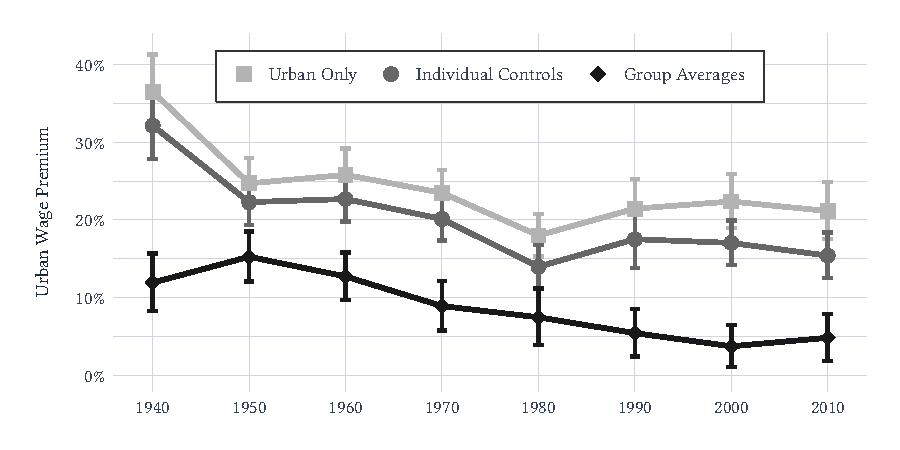
\includegraphics{figures/urban_premium/combined_slides.pdf}
\end{frame}

\begin{frame}{Next slide}
  Hello
\end{frame}


% ------------------------------------------------------------------------------
% \begin{frame}[allowframebreaks]{References}
%   \printbibliography
% \end{frame}
% \appendix
% ------------------------------------------------------------------------------


\end{document}
